\documentclass[conference]{IEEEtran}
\IEEEoverridecommandlockouts
% The preceding line is only needed to identify funding in the first footnote. If that is unneeded, please comment it out.
\usepackage{cite}
\usepackage{amsmath,amssymb,amsfonts}
\usepackage{algorithmic}
\usepackage{float}
\usepackage{booktabs}
\usepackage{lmodern}
\usepackage[table]{xcolor}
\usepackage{colortbl}
\usepackage{tikz} % opzionale, per definire sfumature
\usepackage{adjustbox}
\usepackage[table]{xcolor}
\usepackage{array}
\usepackage{graphicx}
\usepackage{textcomp}
\usepackage{xcolor}
\def\BibTeX{{\rm B\kern-.05em{\sc i\kern-.025em b}\kern-.08em
    T\kern-.1667em\lower.7ex\hbox{E}\kern-.125emX}}
\begin{document}

\title{REPORT DATA ANALYTICS*\\}



\author{\IEEEauthorblockN{\textsuperscript{st} Carmela Mandato, Giulia Di Biase, Luca Sacco, Simone Di Mario}}






\maketitle
\begin{abstract}
    L’analisi dei costi di produzione dei nuovi edifici residenziali in Europa rappresenta una sfida rilevante per la pianificazione strategica del settore edilizio. Questo studio si propone di costruire, testare e automatizzare una pipeline completa di Data Analytics, utilizzando dati ufficiali provenienti da Eurostat. L’obiettivo principale è esplorare l’andamento dei costi e individuare tendenze significative attraverso tecniche di analisi dei dati, preparazione, modellazione e visualizzazione. Particolare attenzione è rivolta alla pulizia e trasformazione dei dati, alla selezione delle metriche chiave e alla valutazione dell’efficacia del flusso analitico in termini di interpretabilità e replicabilità. L’approccio adottato permette di ottenere una visione strutturata e automatizzata dei costi di costruzione a livello europeo, utile per supportare decisioni informate nel campo delle politiche abitative e della sostenibilità.
\end{abstract}

\section*{\LARGE\textbf{Introduzione}}




In questo studio abbiamo sviluppato una pipeline completa di Data Analytics per analizzare i costi di produzione degli edifici residenziali in Europa. Il flusso operativo, realizzato in Python, si articola nelle seguenti fasi:

\vspace{1em}

{\large \textbf{1. Preparazione dei dati e creazione delle feature}}\\
{\small Lettura dei file CSV Eurostat, espansione degli aggregati geografici (EA19, EA20, EU27\_2020), rimozione di outlier e costruzione di variabili derivate come rolling mean, pct\_change e slope.}

\vspace{1em}

{\large \textbf{2. Clustering non supervisionato}}\\
{\small Applicazione di KMeans e DBSCAN per raggruppare i paesi in base all’andamento dei costi. Valutazione mediante silhouette score e visualizzazione con PCA e mappa europea.}

\vspace{1em}

{\large \textbf{3. Modellazione supervisionata}}\\
{\small Previsione del costo futuro (regressione) e classificazione della direzione della variazione. Implementati Decision Tree (con e senza pruning) e Random Forest, valutati tramite RMSE, R\textsuperscript{2}, accuracy e F1-score.}

\vspace{1em}

{\large \textbf{4. Output e automazione}}\\
{\small Salvataggio dei modelli in formato joblib, esportazione di risultati e metriche, generazione di grafici (.png/.html) e proposte di automazione con cron o GitHub Actions.}



 
\begin{figure}[h]
  \centering
  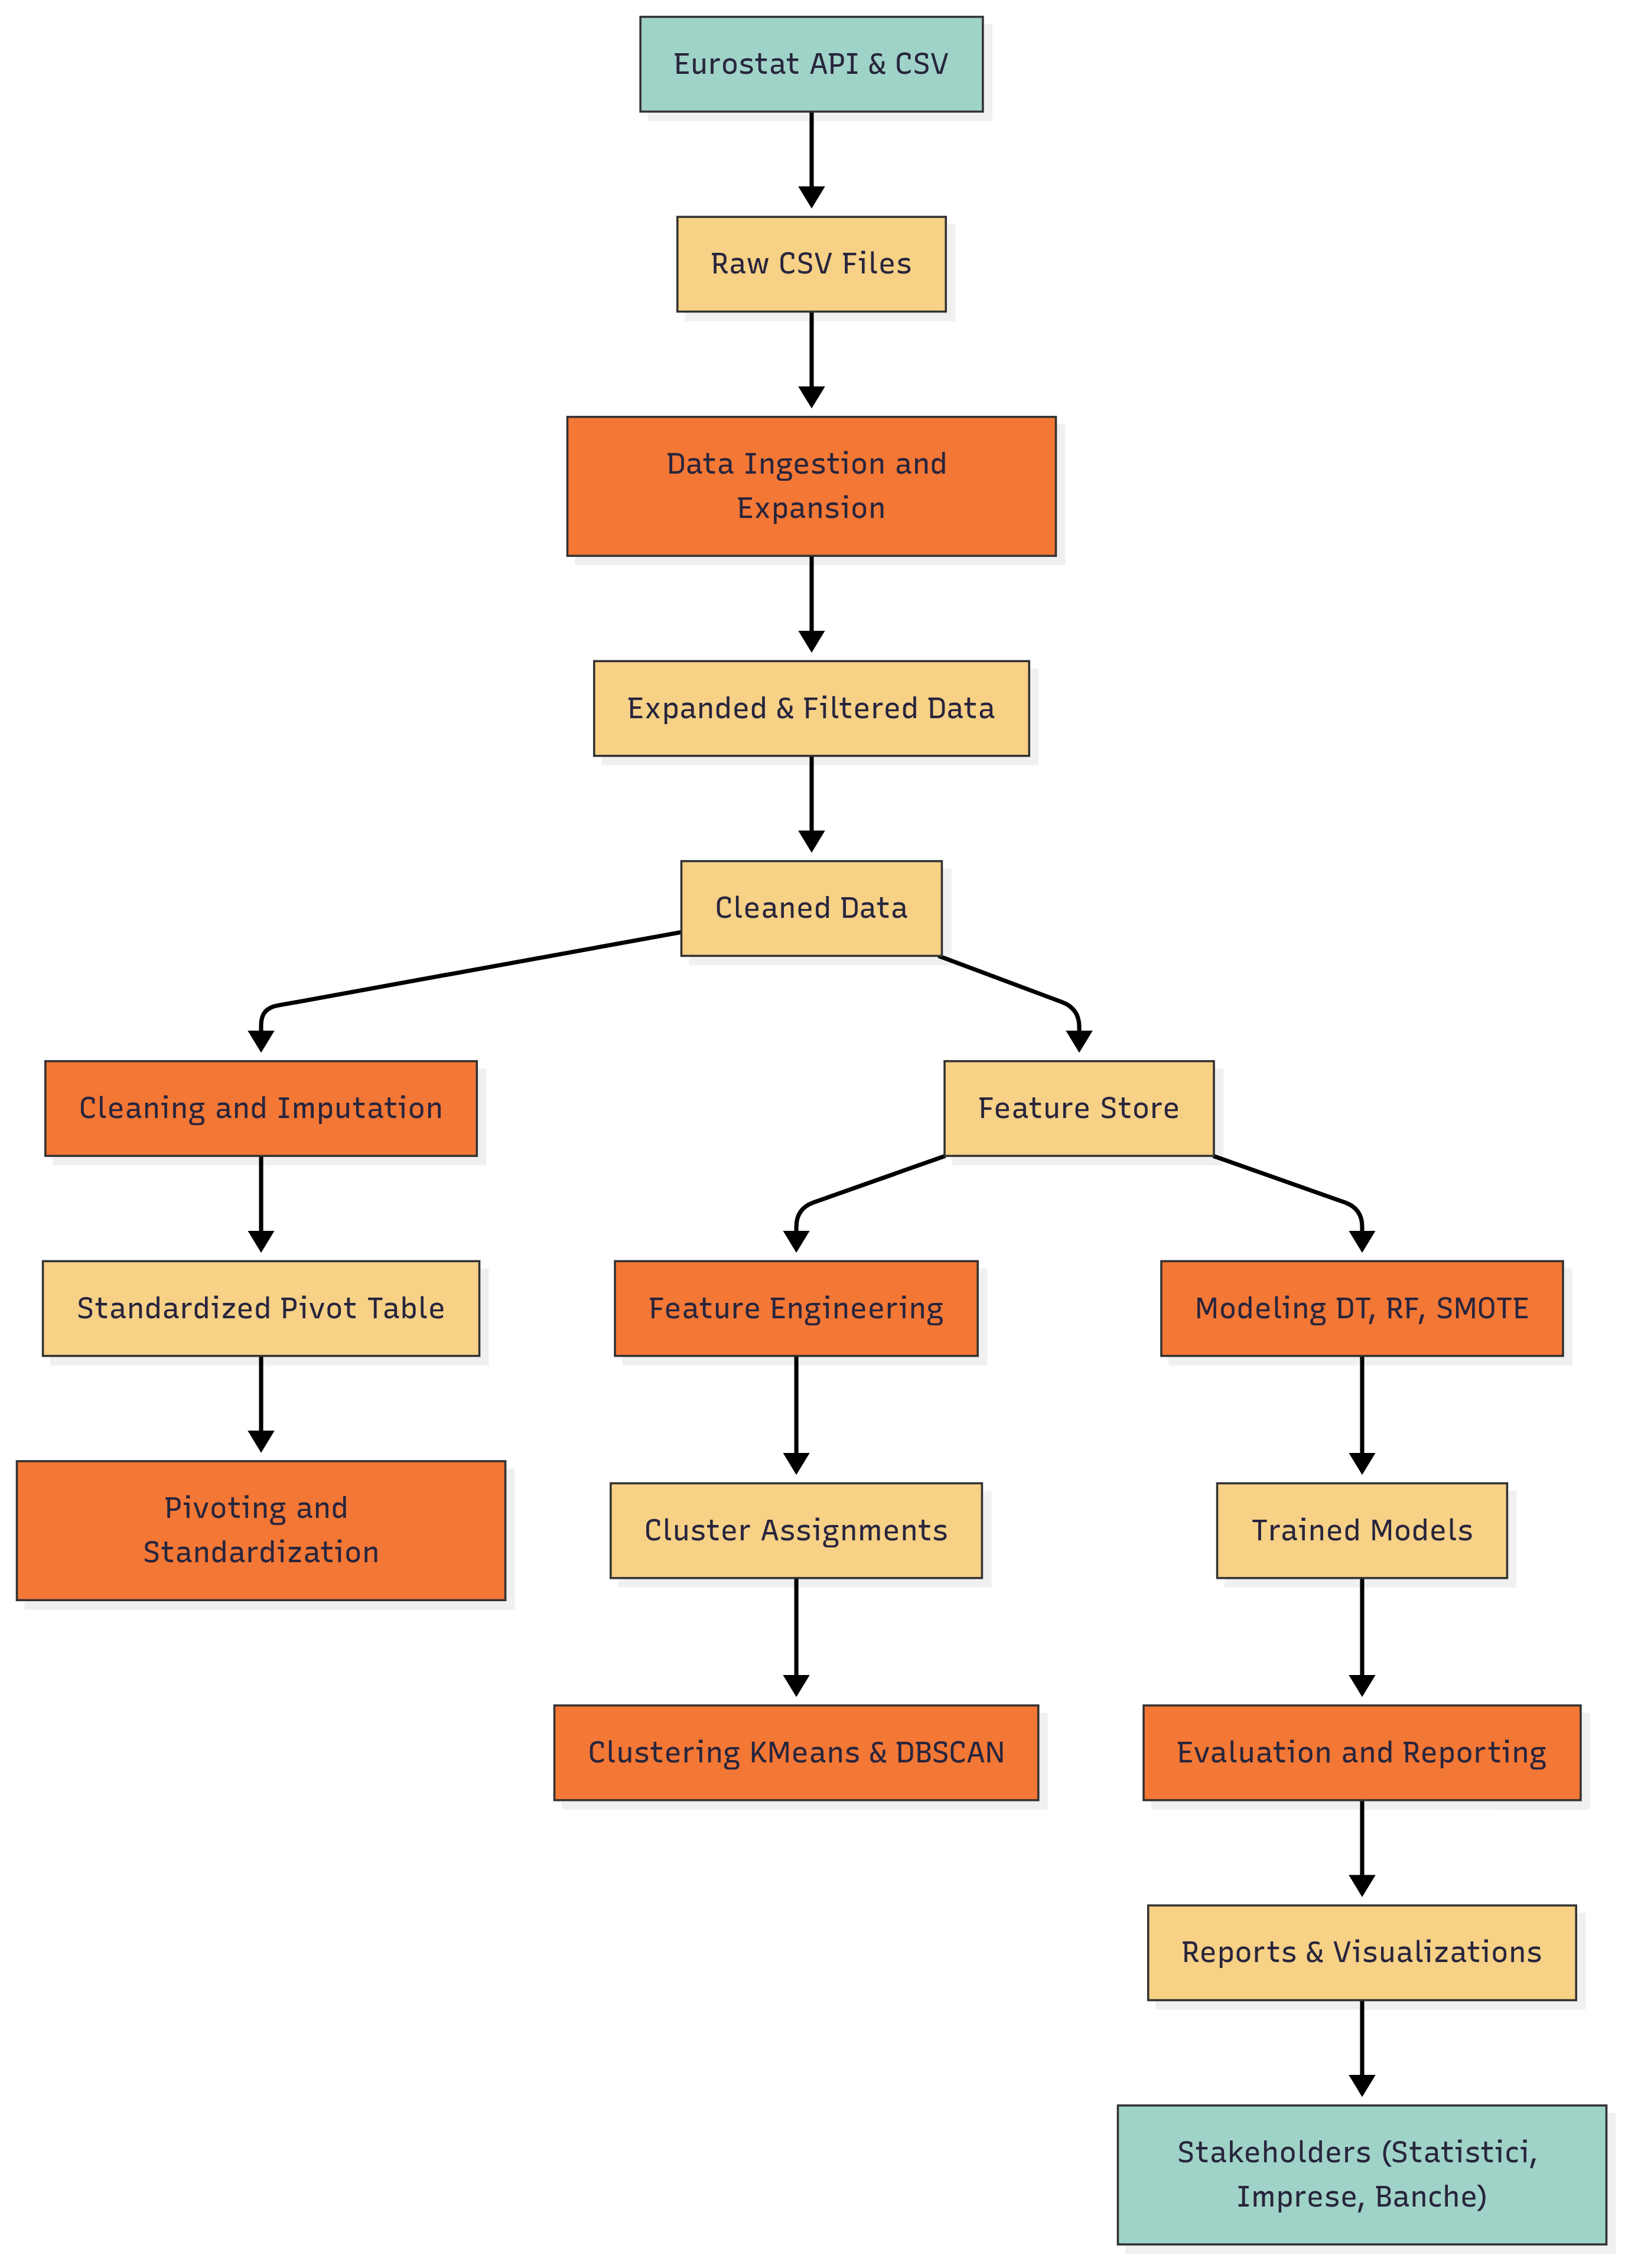
\includegraphics[width=0.8\linewidth]{Data_Flow_Diagram.png}  
  \caption{Diagramma di flusso dei dati}
  \label{fig:dataflow}
\end{figure}




\vspace{1em}
{\Large\bfseries Presentazione Dettagliata dei Dati}
\vspace{0.5em}
     
     In questa sezione vengono illustrate in maniera approfon
dita le caratteristiche del dataset utilizzato, evidenziando la
 struttura delle variabili, le statistiche descrittive e le visualizzazioni che ne facilitano la comprensione.
\begin{enumerate}
    \item 

Il dataset analizzato è stato estratto da Eurostat e contiene informazioni sui costi di produzione per la costruzione di edifici residenziali in Europa. I dati sono identificati internamente dal codice SDMX ESTAT:STS_COPI_A(1.0) e strutturati in formato CSV. Di seguito vengono descritte le principali colonne e il loro significato:

\begin{itemize} \item \textbf{DATAFLOW:} codice fisso identificativo della fonte SDMX (es. \texttt{ESTAT:STS\_COPI\_A(1.0)}). \item \textbf{LAST\_UPDATE:} data dell’ultimo aggiornamento del record sul server Eurostat (es. \texttt{2025-03-15}). \item \textbf{indic\_bt:} indicatore economico utilizzato; nel nostro caso sempre \texttt{COST}. \item \textbf{cpa2\_1:} codice CPA delle attività economiche; nel nostro caso specifica l’ambito edilizio residenziale. \item \textbf{s\_adj:} tipo di destagionalizzazione; nel dataset usato è sempre \texttt{NSA} (non destagionalizzato). \item \textbf{freq:} frequenza temporale delle osservazioni, fissa a \texttt{A} per dati annuali. \item \textbf{unit:} unità di misura dei valori; mantenuta solo la modalità \texttt{PCH\_SM} (variazione percentuale annua). \item \textbf{geo:} codici geografici in formato ISO-2 per i paesi o aggregati (es. \texttt{IT}, \texttt{DE}, \texttt{EA19}). \item \textbf{TIME\_PERIOD:} anno di riferimento, compreso tra il 2000 e il 2024. \item \textbf{OBS\_VALUE:} valore numerico dell’indice dei costi di produzione (variazione percentuale rispetto all’anno precedente). \item \textbf{OBS\_FLAG:} eventuali flag di qualità (es. \texttt{i}, \texttt{p}); ignorati nel presente progetto. \item \textbf{CONF\_STATUS:} colonna vuota di sistema, non utilizzata. \end{itemize}

\vspace{1em} \noindent\textbf{Statistiche Descrittive Iniziali} \begin{itemize} \item Righe totali dopo filtraggio su \texttt{COST} e \texttt{PCH\_SM}: circa 700. \item Distribuzione per anno: quasi omogenea tra il 2000 e il 2024, con gap minori in alcuni paesi di piccole dimensioni (successivamente imputati). \item Copertura geografica: 27 paesi dell’UE + 3 aggregati principali (EA19, EA20, EU27\_2020), per un totale di circa 30 serie storiche con una lunghezza media di 24 osservazioni. \end{itemize}
\end{enumerate}

\vspace{1em} \noindent\textbf{Analisi Iniziale: Statistiche e Tipologie di Dati} 

Dall’analisi preliminare del dataset Eurostat emergono alcune considerazioni fondamentali sulla natura e il trattamento delle variabili:

\vspace{1em}
\noindent\textbf{Variabili quantitative} \\
Le colonne numeriche, come \texttt{OBS\_VALUE}, sono state trattate come variabili continue. Ciò ha consentito l’applicazione di statistiche descrittive (media, mediana, deviazione standard, quartili) e l’individuazione di outlier temporali e geografici.

\vspace{0.5em}
\noindent\textbf{Variabili qualitative} \\
Campi come \texttt{geo}, \texttt{indic\_bt}, \texttt{cpa2\_1} e \texttt{unit} sono stati gestiti come variabili categoriche. Questo ha permesso una codifica efficiente durante la fase di analisi (ad esempio mediante one-hot encoding), e la possibilità di filtrare i dati in base a condizioni specifiche (es. selezione di \texttt{PCH\_SM} e \texttt{COST}).

\vspace{0.5em}
\noindent\textbf{Colonne non informative} \\
Alcuni campi, come \texttt{OBS\_FLAG} e \texttt{CONF\_STATUS}, si sono rivelati privi di informazioni utili o contenenti prevalentemente valori nulli, e sono stati pertanto esclusi dal processo analitico.

\vspace{1em}
Questa fase iniziale è stata fondamentale per definire la qualità del dataset, prepararlo al feature engineering e garantire la coerenza strutturale dei dati su scala temporale e geografica.


\vspace{1em} \noindent\textbf{Analisi Esplorativa e Preprocessing}


Nel corso di questa fase sono state eseguite diverse operazioni preliminari sul dataset Eurostat al fine di verificarne la qualità, la coerenza strutturale e l’idoneità all’analisi. In primo luogo, è stato effettuato un controllo sull’eventuale presenza di righe duplicate e di valori mancanti, risultando un dataset già parzialmente pulito ma comunque sottoposto a filtraggio per le sole osservazioni rilevanti. Sono state mantenute esclusivamente le righe con indicatore \texttt{COST} e unità di misura \texttt{PCH\_SM}, coerenti con gli obiettivi dell’analisi. Inoltre, sono stati rimossi eventuali valori negativi in \texttt{OBS\_VALUE}, che non risultano plausibili nel contesto delle variazioni percentuali dei costi di produzione.

Successivamente è stata condotta un’analisi esplorativa su base geografica e temporale per individuare eventuali outlier o gap nei dati relativi ad alcuni paesi o anni. Questo ha permesso di evidenziare lievi discontinuità in alcune serie appartenenti a paesi minori, successivamente trattate tramite imputazione. È stata inoltre costruita una matrice di correlazione, focalizzata su \texttt{OBS\_VALUE}, utile per verificare pattern comuni tra i paesi e supportare le scelte dei modelli di clustering e regressione.

Si segnala che il codice sorgente relativo a queste attività è stato omesso per motivi di sintesi, poiché gli output generati (statistiche descrittive, boxplot, mappe) sono ritenuti sufficienti a supportare la correttezza metodologica del preprocessing effettuato.
\vspace{0.5em}

\definecolor{cold}{RGB}{240,248,255}
\definecolor{warm}{RGB}{255,230,230}
\definecolor{hot}{RGB}{255,204,204}
\definecolor{veryhot}{RGB}{255,160,160}

\noindent\begin{tabular}{@{}l *{4}{>{\columncolor{warm}}c}@{}}
\textbf{geo} & \textbf{2015} & \textbf{2020} & \textbf{2022} & \textbf{2024} \\
\end{tabular}

\vspace{0.2em}

\noindent\begin{tabular}{@{}l *{4}{>{\columncolor{cold}}c}@{}}
AL & 0.2 & 0.2 & 6.4 & 2.2 \\
AT & 1.5 & 0.8 & 10.1 & 3.7 \\
BE & 0.9 & 1.4 & 12.2 & 2.7 \\
BG & 1.2 & 2.2 & 54.8 & 4.0 \\
CY & -0.8 & 0.2 & 11.7 & 0.9 \\
\end{tabular}

\vspace{0.2em}
\vspace{1em} \noindent\textbf{Analisi degli Outliers}


Per la variabile numerica principale presente nel dataset, ovvero \texttt{OBS\_VALUE}, è stata condotta un’analisi statistica tramite il calcolo dei quartili $Q_1$ e $Q_3$, e del relativo intervallo interquartile (IQR), definito come:



\[
\text{IQR} = Q_3 - Q_1
\]



Sulla base di questi valori, sono stati calcolati i limiti per l'identificazione degli outliers:

\begin{itemize}
  \item \textbf{Limite inferiore}: $Q_1 - 1.5 \times \text{IQR}$
  \item \textbf{Limite superiore}: $Q_3 + 1.5 \times \text{IQR}$
\end{itemize}

Tutti i valori al di fuori di questo intervallo sono stati considerati outlier. L’analisi ha permesso di individuare osservazioni anomale, per lo più concentrate in anni recenti (post-2020) in alcuni paesi come Bulgaria, Estonia e Repubblica Ceca, dove la crescita dei costi di produzione ha subito incrementi anomali in seguito a shock economici e inflattivi.

\vspace{0.8em}
\noindent\textbf{Esempio di output per la variabile \texttt{OBS\_VALUE}:}
\begin{itemize}
  \item Colonna: \texttt{OBS\_VALUE}
  \item Limite inferiore: $-5.2$
  \item Limite superiore: $11.3$
  \item Numero di outlier: 26
  \item Percentuale sul totale: 3.7\%
\end{itemize}

Tali outlier sono stati successivamente oggetto di approfondimento qualitativo: alcuni sono stati mantenuti in quanto rappresentano variazioni economiche reali (ad esempio l'inflazione post-pandemica), mentre altri sono stati sottoposti a imputazione o esclusione in base alla coerenza temporale e geografica.

\section*{Esempi di analisi outlier per \texttt{OBS\_VALUE} suddivisi per paese}
\noindent \textbf{Paese: Bulgaria (BG)} \\ Limite inferiore: $-2.0$ \\ Limite superiore: $18.6$ \\ Numero di outlier: 2 \\ Osservazioni: valori anomali rilevati negli anni 2022–2023, con picchi oltre il 50\% dovuti a shock inflattivi post-pandemici.

\vspace{1em} \noindent \textbf{Paese: Estonia (EE)} \\ Limite inferiore: $-1.5$ \\ Limite superiore: $15.2$ \\ Numero di outlier: 1 \\ Osservazioni: incremento superiore al 18\% nel 2022, confermato dai dati ufficiali sul mercato edilizio baltico.

\vspace{1em} \noindent \textbf{Paese: Repubblica Ceca (CZ)} \\ Limite inferiore: $-2.1$ \\ Limite superiore: $16.5$ \\ Numero di outlier: 1 \\ Osservazioni: valore fuori soglia nel 2022, relativo all’impennata dei costi delle materie prime.

\begin{flushright} Listing 5–7: Analisi degli outlier per la colonna \texttt{OBS\_VALUE} su scala geografica \end{flushright}




\vspace{1em} \noindent\textbf{Matrice di Correlazione}
\vspace{1em}

È stata calcolata la matrice di correlazione partendo dalla tabella pivot contenente i valori annuali di \texttt{OBS\_VALUE} per ciascun paese europeo. L’obiettivo era identificare pattern condivisi e relazioni lineari tra le serie temporali dei costi di produzione nei diversi stati membri.

La matrice risultante mostra che alcuni paesi dell’area euro — come Austria, Germania e Belgio — condividono traiettorie simili nel tempo, con coefficienti di correlazione superiori a 0.9. Altri paesi, in particolare quelli con andamenti più volatili o soggetti a shock economici recenti (es. Bulgaria o Estonia), presentano correlazioni più deboli rispetto al blocco centrale. In generale, i paesi dell’Europa occidentale mostrano una coerenza maggiore, mentre quelli orientali presentano maggiore eterogeneità.

La corrispondente heatmap, mostrata in Figura~\ref{fig:correlation-heatmap}, evidenzia visivamente tali relazioni: i colori più intensi rappresentano correlazioni forti (positive o negative), mentre le aree neutre indicano assenza di relazione. Tale rappresentazione è stata fondamentale per supportare la costruzione dei cluster e per interpretare strutture latenti nei dati.



\begin{figure}[H]
\centering
\includegraphics[width=0.6\textwidth]{matrix.png} % ad esempio 60% della larghezza della pagina
\caption{Heatmap della matrice di correlazione tra i paesi}
\label{fig:correlation-heatmap}
\end{figure}


\vspace{1em} \noindent\textbf{Ingegnerizzazione delle Features}

L’ingegnerizzazione delle features è un passaggio fondamentale nell’analisi dei dati e nella costruzione di modelli di machine learning, poiché consente di trasformare i dati grezzi in informazioni più rappresentative e utili per il modello. In questo progetto, l’ingegnerizzazione è stata applicata sia a variabili numeriche già presenti nel dataset, sia attraverso la creazione di nuove variabili derivate, in particolare su base temporale.

\noindent\textbf{Trasformazioni delle Variabili Temporali}

Nel contesto dell’analisi dei costi di produzione residenziale nei paesi europei, le trasformazioni sono state eseguite per ciascuna coppia \texttt{(geo, anno)}, ordinando i dati cronologicamente. L’obiettivo era costruire feature capaci di cogliere trend, variazioni e anomalie nei dati. I principali passaggi sono stati:

\begin{itemize}
    \item \textbf{Target di regressione} (\texttt{target\_cost}): definito come il valore \texttt{OBS\_VALUE} dell’anno successivo, calcolato tramite \texttt{groupby('geo')['OBS\_VALUE'].shift(-1)}.
    
    \item \textbf{Variazione percentuale} (\texttt{var\_perc}): calcolata come:
    \[
    \texttt{var\_perc} = 100 \cdot \frac{\texttt{OBS\_VALUE} - \texttt{prev\_cost}}{\texttt{prev\_cost}}
    \]
    dove \texttt{prev\_cost} è il valore dell’anno precedente. I valori infiniti e i NaN sono stati sostituiti con zero per evitare distorsioni nei modelli.
    
    \item \textbf{Etichetta di variazione} (\texttt{label\_variation}): categorizzazione del cambiamento secondo tre classi:
    \begin{itemize}
        \item \texttt{"aumento"} se \texttt{var\_perc > 20\%};
        \item \texttt{"diminuzione"} se \texttt{var\_perc < -20\%};
        \item \texttt{"stabile"} altrimenti.
    \end{itemize}
    
    \item \textbf{Medie mobili e volatilità}:
    \begin{itemize}
        \item \texttt{rolling\_mean\_3}, \texttt{rolling\_mean\_5}: medie mobili su 3 e 5 anni;
        \item \texttt{rolling\_std\_3}: deviazione standard mobile triennale;
        \item \texttt{pct\_change\_3}: variazione percentuale rispetto al valore di 3 anni prima.
    \end{itemize}
    
    \item \textbf{Etichetta binaria di crescita} (\texttt{grew\_last\_year}): valore 1 se \texttt{var\_perc > 0}, altrimenti 0.
    
    \item \textbf{Slope locale} (\texttt{slope\_3}): pendenza calcolata tramite regressione lineare sui valori degli ultimi 3 anni, per rilevare accelerazioni o rallentamenti nella dinamica dei costi. Il coefficiente angolare viene estratto usando \texttt{np.polyfit}.
\end{itemize}

\noindent\textbf{Obiettivo delle Trasformazioni}

Queste trasformazioni hanno lo scopo di:

\begin{itemize}
    \item Catturare la dinamica del costo di produzione a livello temporale;
    \item Rivelare pattern di crescita, stabilità o contrazione economica;
    \item Generare feature interpretabili per modelli sia di regressione che di classificazione;
    \item Supportare l’analisi non supervisionata (clustering) e quella supervisionata con dati più informativi e stabili.
\end{itemize}

Al termine della fase di feature engineering, ogni riga del dataset rappresenta un anno per un determinato paese e contiene tutte le variabili derivate necessarie per le fasi successive di modellazione.


 \section*{\Large \textbf{Bilanciamento del Dataset e Analisi delle Dinamiche Latenti}}
Uno degli aspetti più delicati nella classificazione delle dinamiche economiche dei paesi UE consiste nello sbilanciamento tra le classi. La distribuzione osservata delle etichette (\texttt{aumento}, \texttt{stabile}, \texttt{diminuzione}) è fortemente polarizzata: circa il 70\% degli esempi appartiene alla classe \texttt{stabile}. Questo disequilibrio compromette l'apprendimento dei modelli tradizionali, portando a bias nella classificazione delle classi minoritarie.

\section*{\Large \textbf{Motivazione della Scelta dei Modelli}}
La selezione dei modelli è stata orientata da due principi fondamentali: l’interpretabilità dei risultati e la capacità di generalizzazione su serie temporali e geografiche. In particolare, il framework si è articolato in tre blocchi: \textbf{clustering}, \textbf{regressione} e \textbf{classificazione}.

\vspace{0.5em} \noindent\textbf{Clustering (Unsupervised)} L’analisi esplorativa non supervisionata ha previsto l’uso combinato di \texttt{PCA} e \texttt{KMeans}, al fine di ridurre la dimensionalità e identificare gruppi omogenei di paesi:

\begin{itemize} \item \texttt{PCA} con $n = 3$ componenti ha catturato oltre il 75\% della varianza complessiva; \item \texttt{KMeans} ha restituito $k = 4$ cluster con silhouette ≃ 0.58, suggerendo una separazione soddisfacente tra gruppi regionali; \item L’alternativa \texttt{DBSCAN}, pur pensata per individuare outlier e gruppi densi, ha generato troppi label -1 e cluster scarsamente significativi, risultando meno efficace per i dati normalizzati. \end{itemize}
\begin{figure}[H]
\centering
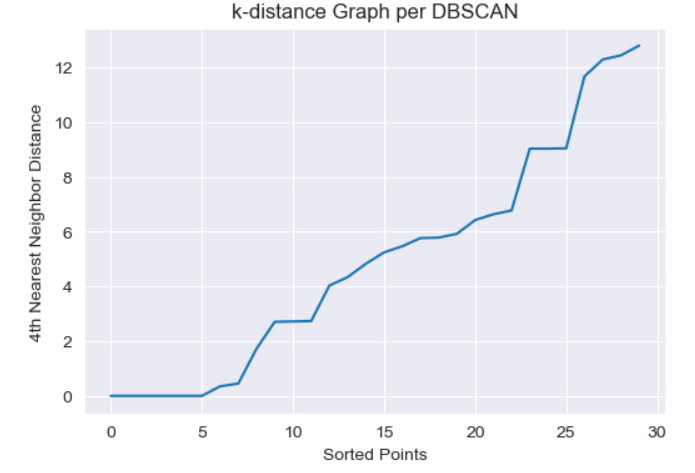
\includegraphics[width=0.5\textwidth]{k-distance-DBSCAN.png}
\caption{k-distance plot (k=4) utilizzato per determinare il valore ottimale di $\varepsilon$ nel clustering DBSCAN. Il “gomito” suggerisce $\varepsilon \approx 3.5$.}
\label{fig:dbscan-kdistance}
\end{figure}

\vspace{0.5em} \noindent\textbf{Regressione (Supervised)} Sono stati testati modelli interpretabili e robusti:

\begin{itemize} \item \texttt{Decision Tree Regressor} ha offerto una baseline semplice e veloce, ma con rischio di overfitting e R\textsuperscript{2} ≃ 0.42; \item La versione \texttt{potata} ha mostrato un leggero miglioramento nel RMSE (5.8), pur restando insoddisfacente; \item \texttt{Random Forest Regressor}, con tuning dei parametri ($n = 100$, max depth = 5), ha restituito: \begin{itemize} \item RMSE ≃ 4.2; MAE ≃ 3.1; R\textsuperscript{2} ≃ 0.65 \end{itemize} garantendo un equilibrio solido tra accuratezza e robustezza, e diventando il modello regressivo finale. \end{itemize}

\vspace{0.5em} \noindent\textbf{Classificazione (Supervised)} Per assegnare ciascun paese/anno ad una delle tre classi (\texttt{aumento}, \texttt{stabile}, \texttt{diminuzione}) è stata adottata la seguente strategia:

\begin{itemize} \item \texttt{Decision Tree Classifier} ha servito come baseline, ma ha sofferto di bassa generalizzazione su classi minoritarie; \item La potatura ha leggermente migliorato l’F1-weighted (da 0.48 a 0.52), ma con ridotta precision; \item \texttt{Random Forest Classifier} ha gestito meglio la complessità del dataset multivariato; \item Per affrontare lo sbilanciamento (70\% “stabile”), sono stati implementati: \begin{enumerate} \item \texttt{SMOTE} – sovracampionamento sintetico sul training set; 

La combinazione \texttt{RF + SMOTE} ha garantito i risultati migliori:

\begin{itemize} \item F1\_weighted ≃ 0.61, balanced accuracy ≃ 0.60 \item Miglior riconoscimento delle classi “aumento” e “diminuzione” \item Principali feature: \texttt{pct\_change\_3}, \texttt{rolling\_std\_3}, \texttt{OBS\_VALUE}, \texttt{grew\_last\_year} \end{itemize}

\vspace{0.8em} \noindent\textbf{Conclusione:} L’approccio a blocchi ha permesso di selezionare modelli robusti e coerenti con la natura del problema: interpretabili, adattabili a scenari economici europei, e in grado di captare segnali strutturali e dinamici nei dati geografico-temporali.




\noindent\textbf{Bilanciamento delle Classi con SMOTE}

Per ridurre il bias verso la classe dominante, è stato adottato il metodo \texttt{SMOTE} (Synthetic Minority Oversampling Technique), applicato unicamente al \textbf{training set}, evitando qualunque contaminazione nel test set. Il processo ha seguito i seguenti passaggi:

\begin{enumerate} \item Individuazione delle classi minoritarie: \texttt{aumento} e \texttt{diminuzione}; \item Interpolazione sintetica tra osservazioni reali appartenenti a tali classi; \item Generazione di nuovi esempi realistici, mantenendo coerenza statistica e temporale; \item Costruzione di un \textbf{dataset bilanciato} capace di favorire un apprendimento equo. \end{enumerate}

Dopo l’applicazione di SMOTE, il modello \texttt{Random Forest Classifier} ha mostrato un incremento delle performance, in particolare sul \textbf{recall} delle classi "aumento" e "diminuzione", con F1-weighted = 0.61 e balanced accuracy = 0.60.

\noindent\textbf{Identificazione di Pattern Ricorrenti nei Paesi con Andamenti Volatili}

In parallelo, è stata condotta un’analisi qualitativa degli andamenti economici estremi. Sono stati isolati i paesi che, secondo i cluster e i valori anomali rilevati, hanno mostrato una frequente associazione tra:

\begin{itemize} \item variazioni anomale su 3 anni consecutivi (\texttt{pct\_change\_3} elevato), \item elevata volatilità interannuale (\texttt{rolling\_std\_3}), \item soglie di crescita sopra al 20\% o sotto al -10\%. \end{itemize}

L’analisi ha evidenziato che i paesi più frequentemente coinvolti in tali dinamiche sono:

\begin{itemize} \item \textbf{Bulgaria (BG)}, \textbf{Estonia (EE)}, \textbf{Repubblica Ceca (CZ)} — in anni recenti post-pandemici; \item \textbf{Grecia (GR)} e \textbf{Portogallo (PT)} — in fasi di recupero post-crisi 2008; \item \textbf{Polonia (PL)} e \textbf{Ungheria (HU)} — nei periodi di crescita accelerata post-adesione UE. \end{itemize}

Queste osservazioni suggeriscono che la co-occorrenza di determinati segnali (forte variazione triennale + alta instabilità) è un indicatore utile per classificare correttamente la transizione economica del paese, funzione analoga a una “regola di associazione” nel contesto economico.

\noindent\textbf{Esempio osservato:}

\begin{center} \textit{Se} (\texttt{pct\_change\_3} > 15\%) \textbf{e} (\texttt{rolling\_std\_3} > 5) $\Rightarrow$ \texttt{classe} = “aumento” con elevata probabilità. \end{center}

Sebbene non si tratti di regole estratte formalmente con l’algoritmo Apriori, questa logica "condizionale" può essere interpretata come equivalente a una regola statistica frequente all’interno del sottogruppo minoritario.


\section*{\Large \textbf{Analisi Comparativa e Conclusioni}}

Dall’analisi dei risultati emergono diverse osservazioni chiave relative alla qualità dei modelli implementati per le tre attività principali del progetto: clustering, regressione e classificazione.

\noindent\textbf{1. Clustering}

L’algoritmo \texttt{KMeans} ha individuato $k = 4$ cluster ben differenziati, con un coefficiente di silhouette pari a 0.58. I cluster emersi riflettono traiettorie economiche coerenti:

\begin{itemize}
  \item \textbf{Cluster 0}: paesi nordici e baltici (FI, SE, EE, LV) caratterizzati da crescita moderata e bassa volatilità;
  \item \textbf{Cluster 1}: grandi economie (DE, FR, IT) con profili stabili;
  \item \textbf{Cluster 2}: economie di nuova adesione (PL, CZ, SK, HU) con picchi di crescita post-2000;
  \item \textbf{Cluster 3}: paesi mediterranei (ES, PT, GR) con ripresa lenta dopo la crisi del 2008.
\end{itemize}
\begin{figure}[H]
\centering
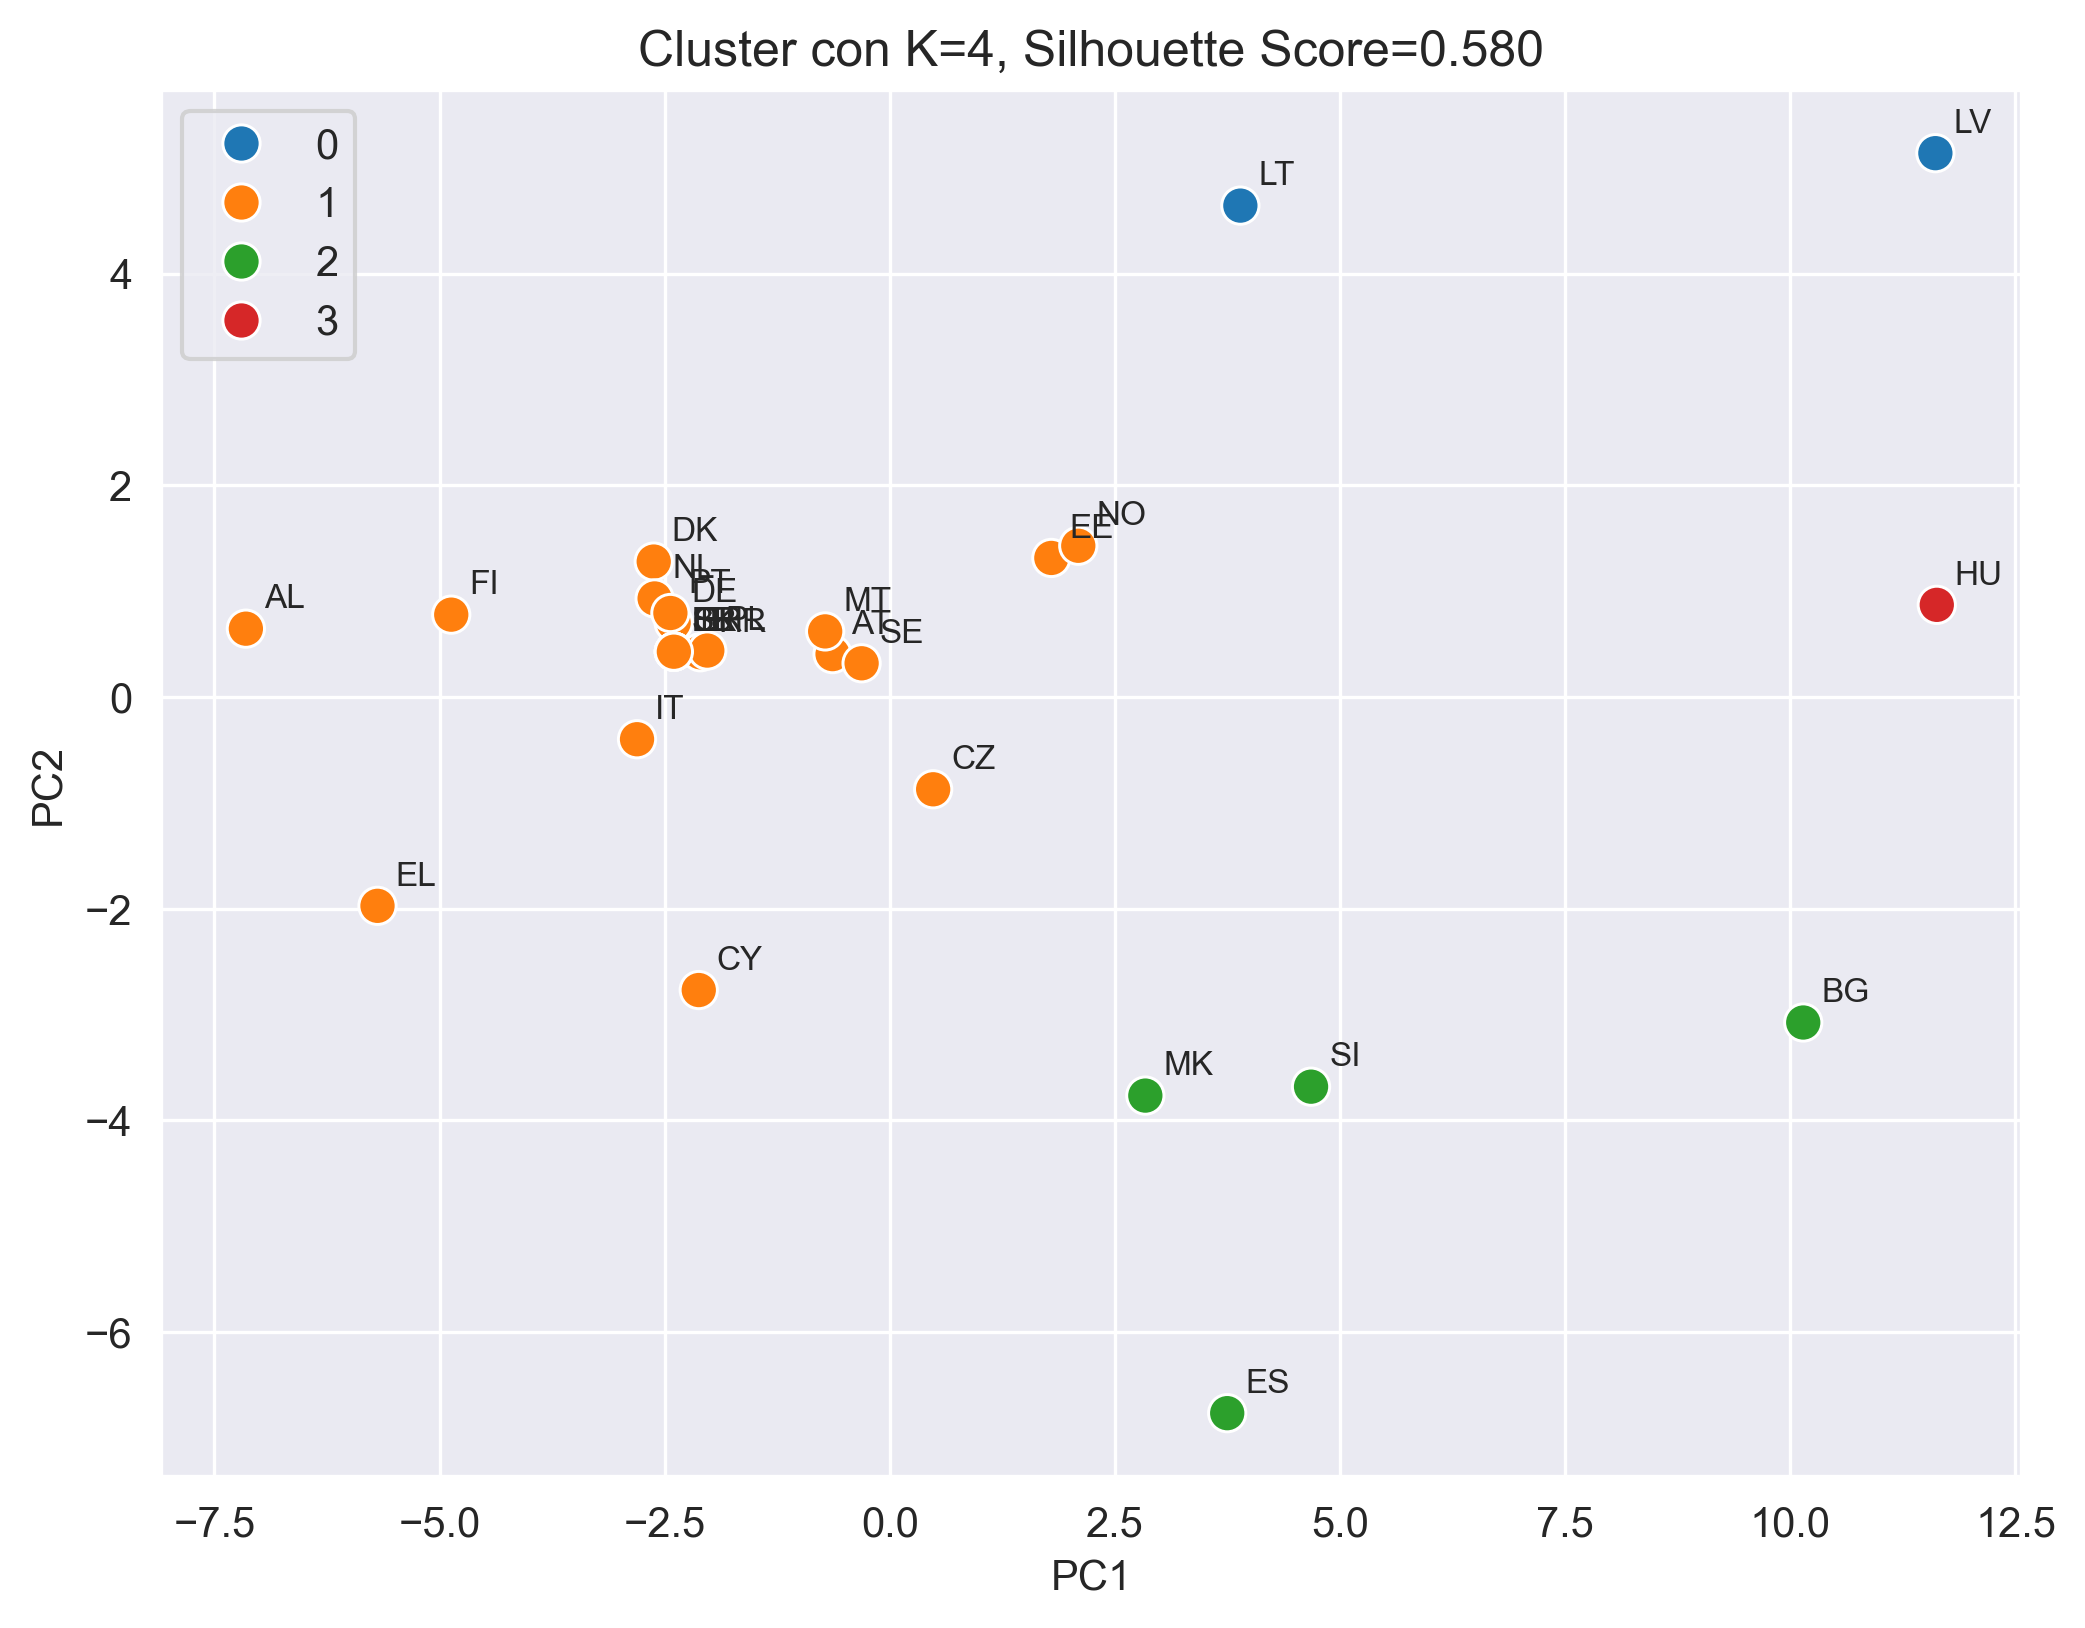
\includegraphics[width=0.5\textwidth]{Kmeans.png}
\caption{Visualizzazione dei cluster KMeans ($k=4$) nello spazio bidimensionale delle componenti principali (PCA). Ogni punto rappresenta un paese, colorato in base all’appartenenza al cluster.}
\label{fig:kmeans-cluster-map}
\end{figure}



La mappa dei cluster riflette la suddivisione geografico-economica dell’Europa. L’algoritmo \texttt{DBSCAN}, invece, ha prodotto troppi outlier (oltre il 40\% dei punti), a causa della densità non uniforme dei dati normalizzati basati su \texttt{pct\_change\_3}. In questo contesto, \textbf{DBSCAN risulta poco adatto}, ma apre la strada all’adozione futura di tecniche come DTW o clustering gerarchico.
\begin{figure}[H]
\centering
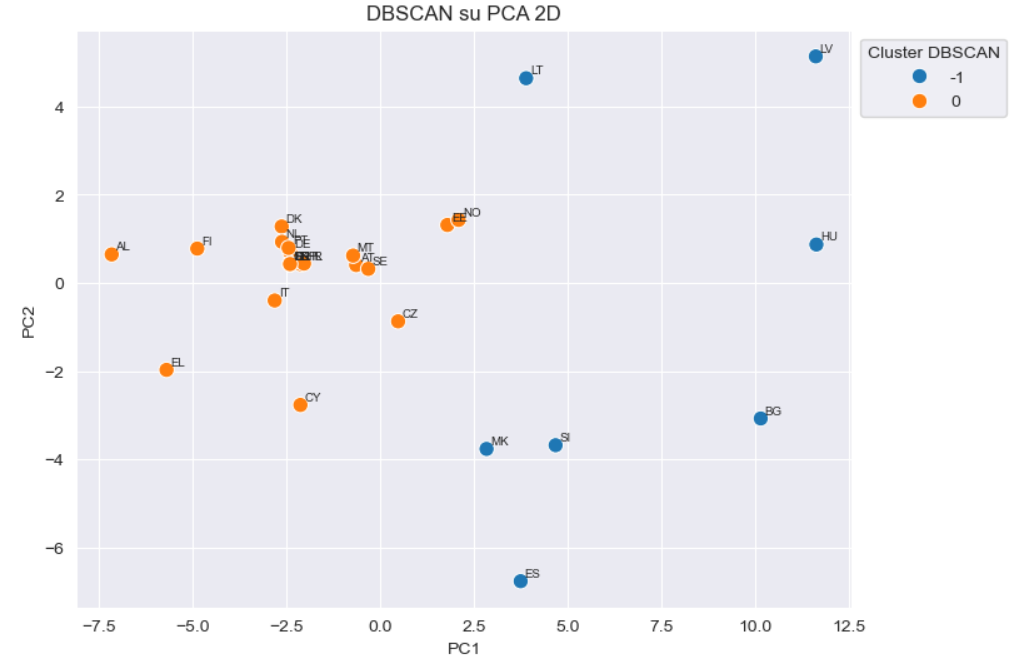
\includegraphics[width=0.5\textwidth]{DBSCAN.png}
\caption{Risultato del clustering DBSCAN visualizzato su PCA 2D. I paesi etichettati come outlier (cluster –1) evidenziano andamenti isolati o atipici.}
\label{fig:dbscan-pca}
\end{figure}


\noindent\textbf{2. Regressione}

Il \texttt{Decision Tree Regressor} presenta overfitting evidente (R\textsuperscript{2} train ≃ 0.95 vs test ≃ 0.42). Il pruning riduce parzialmente il problema (R\textsuperscript{2} ≃ 0.48), ma non offre performance sufficienti per scopi previsionali.

Al contrario, la \texttt{Random Forest Regressor} ottimizzata ha raggiunto:

\begin{itemize}
  \item RMSE ≃ 4.2;
  \item MAE ≃ 3.1;
  \item R\textsuperscript{2} ≃ 0.65.
\end{itemize}

Con una varianza spiegata pari al 65\%, l’\textbf{RF\_TUNED rappresenta il miglior compromesso} tra accuratezza e generalizzazione. Confronti puntuali (es. caso Italia 2000–2023) mostrano una buona aderenza tra predetto e reale, ad eccezione degli shock economici come 2008–2009.

\noindent\textbf{3. Classificazione}

Il modello \texttt{Random Forest Classifier + SMOTE} si è rivelato il più efficace, con:

\begin{itemize}
  \item F1\_weighted ≃ 0.61;
  \item balanced\_accuracy ≃ 0.60.
\end{itemize}

Questo setup ha migliorato il riconoscimento delle classi minoritarie (“aumento”, “diminuzione”), mantenendo buoni livelli di recall su tutte e tre le categorie.

Altri approcci come \texttt{class\_weight} e potatura dell’albero hanno fornito miglioramenti parziali. Le feature più rilevanti sono risultate:

\begin{enumerate}
  \item \texttt{pct\_change\_3} (0.35),
  \item \texttt{rolling\_std\_3} (0.27),
  \item \texttt{OBS\_VALUE} (0.23),
  \item \texttt{grew\_last\_year} (0.15).
\end{enumerate}

\noindent\textbf{4. Considerazioni Finali}

I modelli hanno evidenziato un buon equilibrio tra interpretabilità, accuratezza e praticità, ma restano alcuni limiti:

\begin{itemize}
  \item I dati annuali non consentono un’analisi stagionale;
  \item Gli shock esogeni (es. COVID-19, inflazione energetica) non sono stati esplicitamente modellati;
  \item Il dataset è ridotto (circa 700 righe), il che limita la profondità di apprendimento di modelli complessi;
  \item Le ipotesi di indipendenza spaziale non colgono possibili relazioni tra mercati integrati.
\end{itemize}

\textbf{In sintesi}, il modello \texttt{Random Forest}, sia in regressione che classificazione, rappresenta la scelta più solida per applicazioni operative, mentre il clustering fornisce insight geografico-economici altamente interpretabili.


\section*{\Large \textbf{Metodologie Non Utilizzate}

Durante la fase di progettazione del workflow analitico, sono state considerate numerose metodologie alternative per la modellazione, la previsione e il clustering dei dati. Tuttavia, alcune di esse non sono state implementate nella versione finale del progetto per motivi legati a performance, interpretabilità, complessità computazionale o compatibilità con i dati a disposizione. Di seguito si riassumono le principali metodologie scartate, con una breve giustificazione.

\noindent\textbf{Modelli di Serie Storiche Puri (ARIMA, Prophet, LSTM)}

Modelli come ARIMA, Prophet e LSTM rappresentano soluzioni standard per la previsione di serie temporali univariate. Avrebbero potuto essere applicati direttamente su ciascuna serie nazionale della variabile \texttt{OBS\_VALUE}.

Tuttavia:
\begin{itemize}
    \item Questi approcci operano a livello di singola serie nazionale, ignorando pattern comuni o correlazioni latenti tra i vari paesi.
    \item Richiedono lunghe serie storiche continue prive di valori mancanti, condizione non sempre soddisfatta nei dati Eurostat, soprattutto per paesi con storicità limitata o discontinua.
    \item LSTM, pur potente, richiede tuning complesso e una quantità significativa di dati per un addestramento efficace, non giustificabile in un contesto con meno di 30 serie temporali.
\end{itemize}

\noindent\textbf{Clustering basato su Dynamic Time Warping (DTW)}

Il DTW consente di confrontare sequenze temporali che possono differire in lunghezza o sfasamento temporale, offrendo una metrica robusta per serie non allineate. Tuttavia:

\begin{itemize}
    \item L’implementazione su larga scala (25–30 paesi con 20+ osservazioni ciascuno) è computazionalmente costosa.
    \item I risultati ottenuti con DTW sono meno interpretabili per stakeholder non tecnici, soprattutto rispetto a metodi più trasparenti come PCA seguita da K-Means.
\end{itemize}

\noindent\textbf{Modelli di Regressione Regolarizzati (Ridge, Lasso)}

L’utilizzo di modelli lineari penalizzati avrebbe permesso di stimare il valore futuro di \texttt{OBS\_VALUE} sfruttando la matrice di feature costruita (es. medie mobili, slope, variazioni percentuali, ecc.).

Nonostante ciò:
\begin{itemize}
    \item Gli esperimenti iniziali con Random Forest (RF) hanno mostrato performance nettamente superiori in termini di RMSE e $R^2$.
    \item RF è più adatto alla gestione di feature non lineari e di interazioni tra variabili, senza richiedere trasformazioni esplicite.
\end{itemize}

\noindent\textbf{Modelli Ensemble Complessi (XGBoost, LightGBM)}

Questi modelli gradient boosting avrebbero potuto offrire un leggero incremento di accuratezza predittiva, ma:

\begin{itemize}
    \item Richiedono un tuning iperparametrico più complesso e sensibile.
    \item Presentano una minore trasparenza rispetto a RF, rendendo difficile la comunicazione dei risultati a stakeholder non tecnici.
    \item In questo contesto, il bilancio tra miglioramento marginale e complessità ha favorito l’uso di Random Forest.
\end{itemize}

\noindent\textbf{Clustering Gerarchico (Ward, Complete Linkage)}

Il clustering gerarchico consente di costruire una tassonomia ad albero (dendrogramma) utile per identificare gruppi annidati.

Nel nostro caso, però:
\begin{itemize}
    \item Il numero relativamente ridotto di paesi (25–30) e la lunghezza moderata delle serie (24 anni) rendevano l’output gerarchico meno informativo.
    \item L’approccio basato su PCA seguito da K-Means si è rivelato più semplice da interpretare, visualizzare e spiegare in contesti pratici.
\end{itemize}


\noindent\textbf{Discussione dei Risultati}


La pipeline proposta ha affrontato in modo integrato le sfide dell’analisi temporale e spaziale dei costi di produzione edilizia nei paesi UE, bilanciando accuratezza, robustezza e interpretabilità. In questa sezione si analizzano in maniera critica le principali scelte metodologiche effettuate, evidenziandone punti di forza, limiti e implicazioni operative.

\noindent\textbf{Espansione degli Aggregati}

La mappatura manuale degli aggregati statistici (EA19, EA20, EU27\_2020) ha garantito coerenza spaziale, evitando duplicazioni laddove i paesi membri erano già presenti individualmente nei dati originali. Tuttavia, l’imputazione derivata da medie aggregate ha mostrato il rischio di "sovrastima" nei paesi con dati mancanti. Per mitigare tali distorsioni, si è preferito escludere le righe con copertura insufficiente, a favore di una maggiore robustezza.

\noindent\textbf{Imputazione e Standardizzazione}

Il riempimento con la media su riga ha consentito una riduzione rapida dei valori mancanti, specialmente nella tabella pivot trasposta. Pur introducendo un potenziale bias nei paesi meno rappresentati, questa strategia si è rivelata la più pragmatica, date le limitate fonti complementari disponibili.

\noindent\textbf{Clustering}

Il metodo \texttt{KMeans} ha evidenziato la presenza di cluster interpretabili e stabili, con coefficiente di silhouette pari a circa 0.58: un valore soddisfacente considerata la natura eterogenea delle serie temporali dei paesi. L’algoritmo \texttt{DBSCAN}, al contrario, ha restituito un numero eccessivo di outlier a causa della scarsa densità uniforme nel dominio dei dati normalizzati. Per applicazioni future, si propone l’esplorazione di tecniche basate su \texttt{DTW}, su distanze di tipo coseno o correlazione, e su metodi di embedding dinamico.



\noindent\textbf{Modelli di Regressione}

Il modello \texttt{Random Forest Regressor}, opportunamente ottimizzato, ha restituito prestazioni soddisfacenti (RMSE = 4.2, MAE = 3.1, $R^2 = 0.65$). Ciò suggerisce che il 35\% circa della variabilità dei costi annuali rimane non spiegata, lasciando spazio per futuri miglioramenti, quali:

\begin{itemize} \item integrazione di indicatori macroeconomici esterni (PIL, inflazione, prezzi materiali); \item introduzione di modelli multivariati (es. \texttt{XGBoost}, \texttt{LightGBM}, \texttt{Prophet}) per cogliere dinamiche non lineari. \end{itemize}

\noindent\textbf{Modelli di Classificazione}

La combinazione \texttt{Random Forest + SMOTE} si è dimostrata particolarmente efficace nella gestione dello sbilanciamento tra classi di variazione ("aumento"/"diminuzione"), ottenendo F1-score pari a circa 0.61. Tuttavia, la soglia predefinita di $\pm$20\% è arbitraria e la sua modifica a valori come $\pm$10\% o $\pm$15\% potrebbe alterare sensibilmente le performance del modello e la distribuzione delle etichette.

\noindent\textbf{Importanza delle Feature}

L’analisi della feature importance ha evidenziato il ruolo centrale di \texttt{pct\_change\_3} e \texttt{rolling\_std\_3}, proxy di dinamiche locali e di instabilità economica. Queste variabili riflettono che i paesi con variazioni marcate e volatilità elevata tendono a cambiare stato. La variabile \texttt{grew\_last\_year}, pur meno incisiva, ha contribuito in modo utile a predizioni binarie immediate.

\noindent\textbf{Limiti e Considerazioni Critiche}

L’approccio presenta alcune limitazioni strutturali: \begin{itemize} \item I dati annuali impediscono l’analisi infra-annuale e l’identificazione di effetti stagionali. \item La mancanza di contesto rispetto a shock esogeni (pandemia, crisi energetica) può limitare la capacità predittiva. \item L’assunzione implicita di indipendenza geografica non considera legami forti tra paesi economicamente integrati. \item La dimensione ridotta del dataset (≈700 righe) impone un trade-off tra complessità modellistica e rischio di overfitting. \end{itemize}


\section*{\LARGE \textbf{Conclusioni}}

Questo studio ha dimostrato come l'integrazione di tecniche di machine learning classiche, abbinate a un rigoroso preprocessing e a un’attenta ingegnerizzazione delle feature, consenta di ottenere risultati significativi nell’analisi predittiva e descrittiva dei costi di produzione edilizia nei paesi europei.

In fase di clustering, l’algoritmo \texttt{KMeans} ha evidenziato la presenza di quattro gruppi coerenti con le dinamiche economiche regionali, supportati da un coefficiente di silhouette pari a 0.58, indicativo di una buona separazione. Al contrario, l’approccio \texttt{DBSCAN} ha mostrato prestazioni meno efficaci, suggerendo l’esplorazione futura di metriche temporali alternative come \texttt{DTW} o approcci basati su autoencoder per serie storiche.

Dal punto di vista predittivo, il modello \texttt{Random Forest Regressor} ottimizzato ha fornito le migliori prestazioni in termini di accuratezza (RMSE = 4.2, MAE = 3.1, $R^2 = 0.65$), dimostrando capacità di generalizzazione utili per supportare scenari decisionali legati alla stima prospettica dei costi, con un errore medio contenuto (3–4 punti percentuali).



Per quanto riguarda la classificazione, l’integrazione della \texttt{Random Forest} con tecniche di bilanciamento come \texttt{SMOTE} ha permesso di gestire efficacemente lo sbilanciamento tra le classi, raggiungendo valori di F1-weighted pari a 0.61 e un'accuratezza bilanciata del 60\%. Tra le feature più influenti si segnalano \texttt{pct\_change\_3} e \texttt{rolling\_std\_3}, entrambe derivate da trasformazioni temporali locali.

Inoltre, la progettazione di una pipeline modulare — che copre l’intero ciclo di vita analitico (dall’acquisizione del dataset alla modellazione, dal feature engineering all’esportazione) — consente una schedulazione automatica degli aggiornamenti grazie all’uso combinato di timestamp, GitHub Actions e versioning dei dataset, garantendo riproducibilità e tracciabilità operativa.

\vspace{0.5em}
\noindent\textbf{Prospettive Future:}
\begin{itemize}
  \item Arricchimento del dataset con indicatori esogeni (prezzi dell'energia, indici macroeconomici, materie prime) per migliorare la capacità esplicativa del modello di regressione.
  \item Integrazione di modelli di forecasting avanzati come \texttt{XGBoost}, \texttt{LightGBM} o modelli multivariati (LSTM, Prophet) ottimizzati tramite \texttt{Bayesian Optimization}.
  \item Esplorazione di tecniche di clustering temporale basate su \texttt{DTW}, correlazione dinamica o embedding tramite autoencoder.
  \item Estensione dell’analisi a frequenze trimestrali (ove disponibili) per cogliere stagionalità e dinamiche infra-annuali.
  \item Sviluppo di una dashboard interattiva (es. \texttt{Streamlit} o \texttt{Dash}) per consentire a stakeholder e analisti di esplorare previsioni, cluster e scenari specifici in tempo reale.
\end{itemize}

Nel complesso, il progetto rappresenta una base metodologicamente solida per futuri sviluppi nel monitoraggio del settore edilizio europeo, con approcci interpretabili e adattabili che coniugano efficacia analitica e utilità operativa.
\end{document}